\documentclass[12pt]{article}\usepackage[]{graphicx}\usepackage[]{color}
%% maxwidth is the original width if it is less than linewidth
%% otherwise use linewidth (to make sure the graphics do not exceed the margin)
\makeatletter
\def\maxwidth{ %
  \ifdim\Gin@nat@width>\linewidth
    \linewidth
  \else
    \Gin@nat@width
  \fi
}
\makeatother

\definecolor{fgcolor}{rgb}{0.345, 0.345, 0.345}
\newcommand{\hlnum}[1]{\textcolor[rgb]{0.686,0.059,0.569}{#1}}%
\newcommand{\hlstr}[1]{\textcolor[rgb]{0.192,0.494,0.8}{#1}}%
\newcommand{\hlcom}[1]{\textcolor[rgb]{0.678,0.584,0.686}{\textit{#1}}}%
\newcommand{\hlopt}[1]{\textcolor[rgb]{0,0,0}{#1}}%
\newcommand{\hlstd}[1]{\textcolor[rgb]{0.345,0.345,0.345}{#1}}%
\newcommand{\hlkwa}[1]{\textcolor[rgb]{0.161,0.373,0.58}{\textbf{#1}}}%
\newcommand{\hlkwb}[1]{\textcolor[rgb]{0.69,0.353,0.396}{#1}}%
\newcommand{\hlkwc}[1]{\textcolor[rgb]{0.333,0.667,0.333}{#1}}%
\newcommand{\hlkwd}[1]{\textcolor[rgb]{0.737,0.353,0.396}{\textbf{#1}}}%

\usepackage{framed}
\makeatletter
\newenvironment{kframe}{%
 \def\at@end@of@kframe{}%
 \ifinner\ifhmode%
  \def\at@end@of@kframe{\end{minipage}}%
  \begin{minipage}{\columnwidth}%
 \fi\fi%
 \def\FrameCommand##1{\hskip\@totalleftmargin \hskip-\fboxsep
 \colorbox{shadecolor}{##1}\hskip-\fboxsep
     % There is no \\@totalrightmargin, so:
     \hskip-\linewidth \hskip-\@totalleftmargin \hskip\columnwidth}%
 \MakeFramed {\advance\hsize-\width
   \@totalleftmargin\z@ \linewidth\hsize
   \@setminipage}}%
 {\par\unskip\endMakeFramed%
 \at@end@of@kframe}
\makeatother

\definecolor{shadecolor}{rgb}{.97, .97, .97}
\definecolor{messagecolor}{rgb}{0, 0, 0}
\definecolor{warningcolor}{rgb}{1, 0, 1}
\definecolor{errorcolor}{rgb}{1, 0, 0}
\newenvironment{knitrout}{}{} % an empty environment to be redefined in TeX

\usepackage{alltt}  
\usepackage{amsfonts, amsmath, amsthm, amssymb, enumitem, verbatim, graphicx}
\setlength{\parindent}{0pt}
\setlength{\parskip}{1ex plus 0.5ex minus 0.2ex}
\usepackage [margin=1in, paperwidth=8.5in, paperheight=11in]{geometry}

\newcommand{\bfbeta}{\mbox{\boldmath $\beta$}}
\newcommand{\bfX}{\mbox{\boldmath $X$}}
\newcommand{\bfx}{\mbox{\boldmath $x$}}
\newcommand{\bfV}{\mbox{\boldmath $V$}}
\newcommand{\bfI}{\mbox{\boldmath $I$}}
\newcommand{\bfy}{\mbox{\boldmath $y$}}
\newcommand{\bfeps}{\mbox{\boldmath $\epsilon$}}
\IfFileExists{upquote.sty}{\usepackage{upquote}}{}
\begin{document}


{ \flushright Jordan Schupbach \\
STAT 532\\
September 11, 2015 \\}
Homework \# 2\\

\begin{enumerate}
\item 
\begin{itemize}
\item Many books define probabilities using the axioms of probabilities (sometimes stated as Kolmogorov's Axioms). In 'Statistical Inference' by Casella and Berger, the authors introduce probabilities with the following definition.\\

Given a sample space $S$ and an associated sigma algebra $\mathcal{B}$, a \emph{probability function} is a function $P$ with domain $\mathcal{B}$ that satisfies
\begin{enumerate}[label= {\bf \arabic*. }]
\item $P(A) \geq 0$ for all $A \in \mathcal{B}.$
\item $P(S) = 1.$
\item If $A_1, A_2, \dots \in \mathcal{B}$ are pairwise disjoint, then $P(\cup_{i=1}^{\infty} A_i ) = \sum_{i=1}^{\infty} P(A_i).$
\end{enumerate}
In the book 'Bayesian Data Analysis (3rd Edition)' by Gelman et al., the authors write this same definition in somewhat simpler terms: 'the mathematical definition of probability: that probabilities are numerical quantities, defined on a set of 'outcomes,' that are nonnegative, additive over mutually exclusive quantities, and sum to 1 over all possible mutually exclusive outcomes.'
\item The word 'probability' has shared many meanings over the course of history, and its specific meaning should be made in the context of when it was said and by whom. Uses of the word originate from two separate goals. One, in describing \emph{uncertainty}, and the other in the process of \emph{induction}. Prior to about 1700, probability was limited to describing the cogency of a declaration. After this, the mathematical definition emerged out of the gambling world and eventually became the dominant use of the word. To further convolute the definition, divisions within the discipline of statistics use the word in different ways. For instance, frequentists restrict its usage to describing a long-run frequency, whereas Bayesians and Likelihoodists accept its usage as a measure of certainty for a single outcome.
\end{itemize} 
\item One criticism of the likelihood principle is that it doesn't take into account experimental design. All of the information regarding the parameter is contained in the likelihood. Thus, two completely different experiments could yield the same inference about a parameter despite having different study designs, so long as both have the same likelihood. To illustrate, consider two experiments of flipping a coin, where the researcher's parameter of interest is $p$, the probability that a single coin flip will result in a ''heads''. In one experiment, call it $E_1$, we flip a coin 12 times and record the number of heads. In the other experiment, $E_2$, we record the number of tails until the third head. We have $E_1$ associated with the family of $binomial(12,p)$ pmfs and $E_2$ associated with the family of $nbinom(3,p)$ pmfs. Now, consider two sample points $x_1 = 3$ (3 out of 12 heads in $E_1$) and $x_2 = 12$ (the third head occurs on the 12th coin flip in $E_2$). We have the following likelihood functions for each experiment
$$L(p|x_1=12) = {12 \choose 3} p^3 (1-p)^{12} \; \text{for } E_1$$
and
$$L(p|x_2=13) = {11 \choose 2} p^3 (1-p)^{12} \; \text{for } E_2$$

Before continuing, we will state the formal likelihood principle:\\

Suppose that we have two experiments, $E_1 = ( \bfX_1, \theta, \{ f_1( \bfx_1 | \theta \})$ and  $E_2 = ( \bfX_2, \theta, \{ f_2( \bfx_2 | \theta \})$, where the unknown parameter $\theta$ is the same in both experiments. Suppose $\bfx_1^*$ and $\bfx_2^*$ are sample points from $E_1$ and $E_2$ respectively, such that
$$L(\theta | \bfx_2^*) = C L(\theta | \bfx_1^*)$$
for all $\theta$ and for some constant $C$ that may depend on $\bfx_1^*$ and $\bfx_2^*$ but not $\theta$.
Then,
\[Ev(E_1, \bfx_1^*) = Ev(E_2, \bfx_2^*)\]
where $Ev(E, \bfx)$ stands for the \emph{evidence about $\theta$ arising from $E$ and $\bfx$}.\\

That is, the formal likelihood principle states that the evidence about $p$ from both experiments with their respective samples should be equal since their likelihoods are proportional. In fact, the MLE in either case is $\hat{p} = \dfrac{3}{12} = .25$.  Suppose the following mixed experiment. A researcher has his colleague flip a coin and carry out $E_1$ if he flips a heads and carry out $E_2$ if he flips a tails. The researcher, unknowing of which experiment was conducted, receives the data of 3 heads out of 12 flips from his colleague. In either case, the researcher concludes that the probability of getting a heads on a single coin flip is .25, however, he does not know whether $3$ or $12$ was the fixed value. The former is an illustration of the formal sufficiency principle and the conditionality principle; which, by Birnbaum's theoerem, is both necessary and sufficient for the formal likelihood principle.\\

Now, let us consider testing the null hypothesis $H_0: p = .5$ versus the alternative $H_a: p < .5$. Given that the null is true, the probability of observing 7 or fewer heads in $E_1$ is 
\begin{align*}
P(X_1 \leq 3 | p = .5, n = 12) &= \left ( {12 \choose 12} + {12 \choose 11} +  {12 \choose 10} +  {12 \choose 9}  \right) \left ( \frac{1}{2} \right )^{12} \\
&= \dfrac{299}{4096} \\
&\approx .073
\end{align*}
In $E_2$, we have the probability of needing to conduct 12 or more experiments is
\begin{align*}
P(X_2 \geq 12 | p = .5, r = 3) &= 1 - P(X_2 \leq 12 | p = .5, r = 3)\\
&= 1 - \left ( {10 \choose 2} \left ( \dfrac{1}{2} \right)^{11} + {9 \choose 2} \left ( \dfrac{1}{2} \right)^{10} + \dots + {2 \choose 2} \left ( \dfrac{1}{2} \right)^3  \right )\\
&= \dfrac{134}{4096}\\
& \approx .0327
\end{align*}

These calculations are the associated p-values of each experiment. Hence, we would reject the null hypothesis in $E_1$ at the .05 confidence level and would fail to reject the null in $E_2$ if we knew which experiment was conducted. Some would say that because of this the likelihood principle is flawed as it doesn't take into account the experimental design. Likelihoodists would likely respond by saying that this simply exemplifies the flaws in significance testing. The arguments within this problem come from 2 sources. The first is in section 6.3.2 in 'Statistical Inference' by Casella and Berger and the second is in the wikipedia page for 'Likelihood.' I am uncertain as to the original source of this problem, however I would suspect that it comes from the debates between Fisher and Neyman.

\item The sampling distribution is related to the likelihood function in that if we fix a sample $\bfX$, then the function of $\theta$ defined by
\[ L(\theta | \bfx) = f(\bfx | \theta) \]
is the likelihood function. Then, if we consider two values of $\theta$, say $\theta_1$ and $\theta_2$, and find that 
\[ P_{\theta_1}( \bfX = \bfx) = L(\theta_1 | \bfx) > L(\theta_2 | \bfx) = P_{\theta_2}(\bfX = \bfx) \]
we find that the value observed sample is more likely to have occured if $\theta = \theta_1$ than if $\theta = \theta_2$. Hence, if we maximize $L(\theta | \bfx)$, we find the most likely value $\theta$ given the sample $\bfx$. Thus, the likelihood function (and by extension, MLE's) is directly related to the sampling distribution through the definition of the likelihood function. 
\item The likelihood function is a function of our parameter of interest for a given sample which tells us how 'likely' a given value of our parameter of interest is, given we observe a specific set of data. To be clear though, we do not mean 'likely' in a strict probabalistic sense. In fact, a likelihood function is not a probability function. First, the sum over all possible values of the likelihood function does not have to be 1. That is, in probabilities, when we consider an experiment, the probability of something happening is 1. If we want to make further statements about what that something is, it might be less than 1 (but greater than zero). In contrast, the sum over the likelihood function can be any nonnegative real number (it might even be infinite). 

\item If we want to estimate survivability of some birds, and one week, all of the birds survived, we might conclude that the probability of all birds surviving any given week is 1. This would effectively mean that these birds are invincible, which we know not to be true. If we use Bayesian methods, situations  such as these are not a problem, as we can simply restrict our prior distribution so that it is impossible to conclude survivability of 1. As pointed out in class, our choice of prior can in some ways be related to increasing our sample size. For instance, choosing a $beta(1,1)$ prior would be equivalent to adding one survived and one died to the sample and choosing a $beta(.5,.5)$ would be equivalent to adding a half to each group. In effect, based on how likely or unlikely we think high (or low) values of survivabililty are in the samples for various sample sizes, we may want to choose an appropriate prior as to not strongly influence the inferences made from the data observed.

\item We get the following plots of the beta distribution for different values of $\alpha = \beta$.

\begin{knitrout}
\definecolor{shadecolor}{rgb}{0.969, 0.969, 0.969}\color{fgcolor}

{\centering 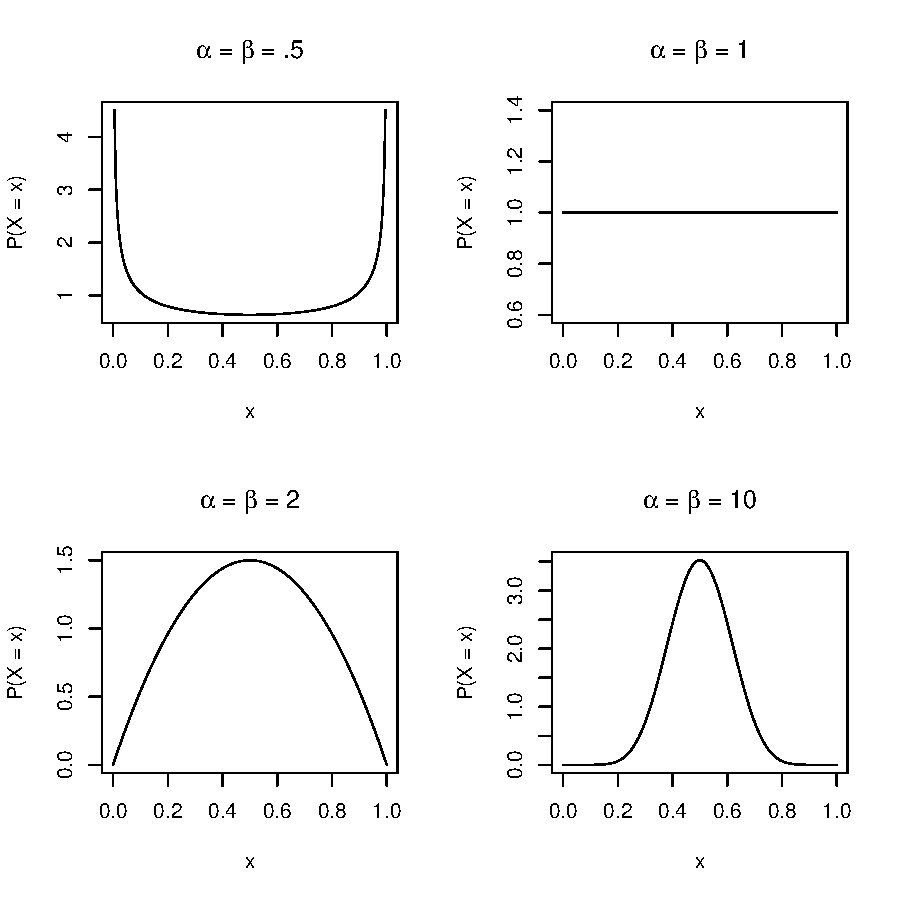
\includegraphics[width=\maxwidth]{figure/plot6-1} 

}



\end{knitrout}

\item We get the following plots of the gamma distribution for different values of $\alpha = \beta$.

\begin{knitrout}
\definecolor{shadecolor}{rgb}{0.969, 0.969, 0.969}\color{fgcolor}

{\centering 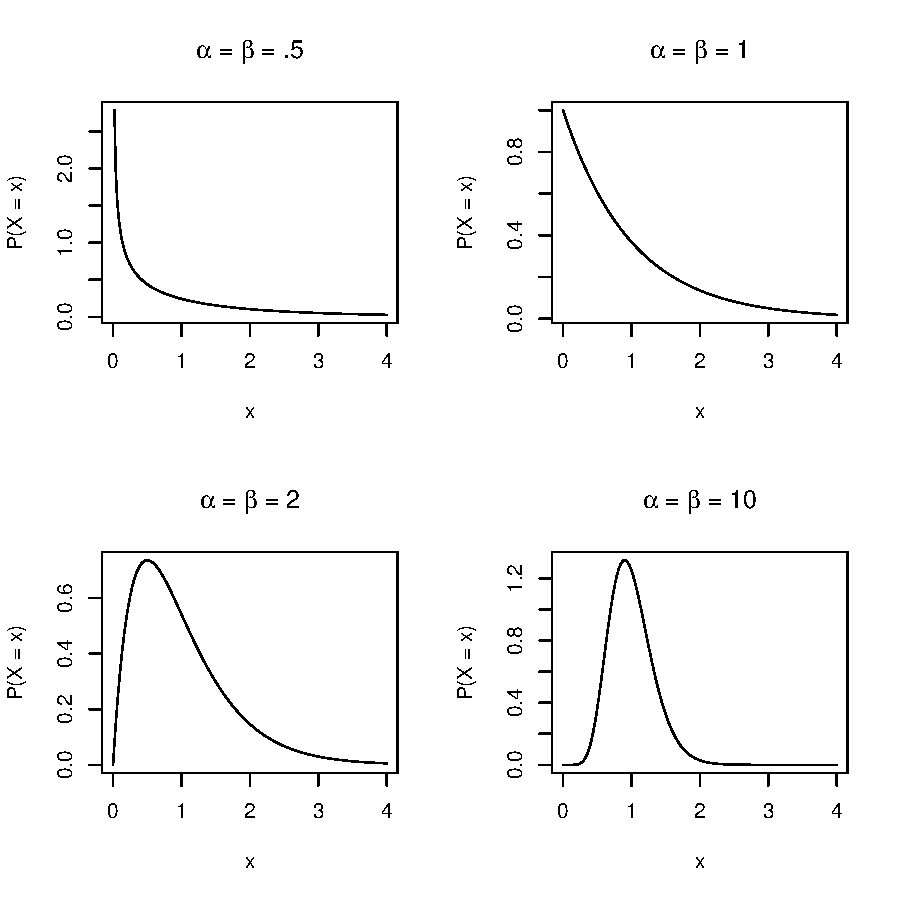
\includegraphics[width=\maxwidth]{figure/plot7-1} 

}



\end{knitrout}

The gamma distribution is often used for the shape parameter for a normal model with mean known and variance unknown as it is the conjugate prior for this distribution. 

\item
\begin{enumerate}[label = (\alph*)]
\item We have 
\[ P(Infect | T \; +) = \dfrac{P(Test \; + | Infect) P(Infect)}{P(T \; + | Infect) P(Infect) + P(T \; + | No \; Infect) P(No \; Infect)}  \]
and so for doctor one, we have
\[ P(Infect | T \; +) = \dfrac{(.92)(.05)}{(.92)(.05) + (.1)(.95)} \approx 0.3262411 \]
and for doctor two, we have
\[ P(Infect | T \; +) = \dfrac{(.92)(.1)}{(.92)(.1) + (.1)(.9)} \approx 0.5054945 \]

\item For both doctor's a beta prior was used based on what was thought of as having reasonable quantiles for each prior belief. A beta() was used for doctor 1 and a beta() was used for doctor 2 as the quantiles associated with each seemed to reasonably reflect their prior beliefs. We draw the priors below.

\begin{knitrout}
\definecolor{shadecolor}{rgb}{0.969, 0.969, 0.969}\color{fgcolor}

{\centering 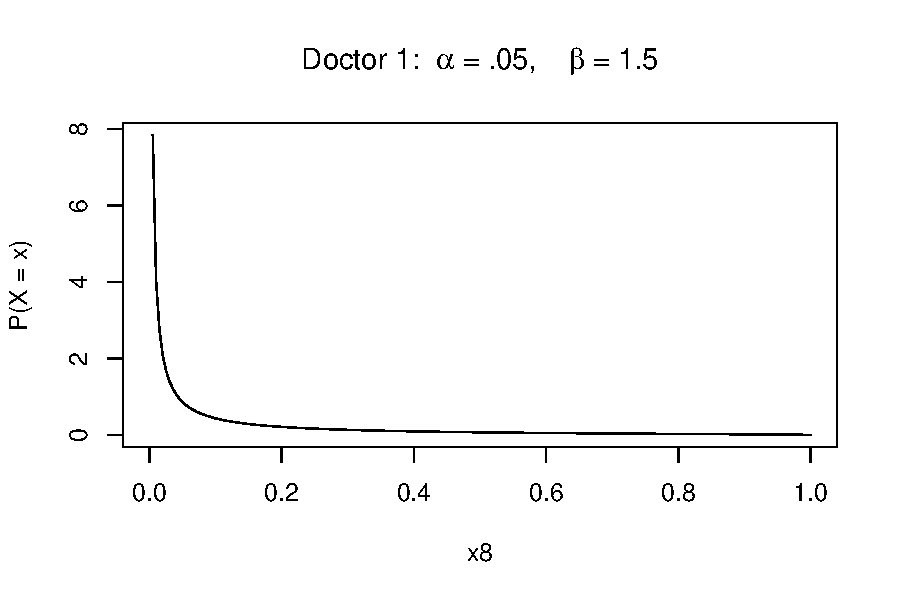
\includegraphics[width=\maxwidth]{figure/plot8a-1} 

}



\end{knitrout}

\begin{knitrout}
\definecolor{shadecolor}{rgb}{0.969, 0.969, 0.969}\color{fgcolor}

{\centering 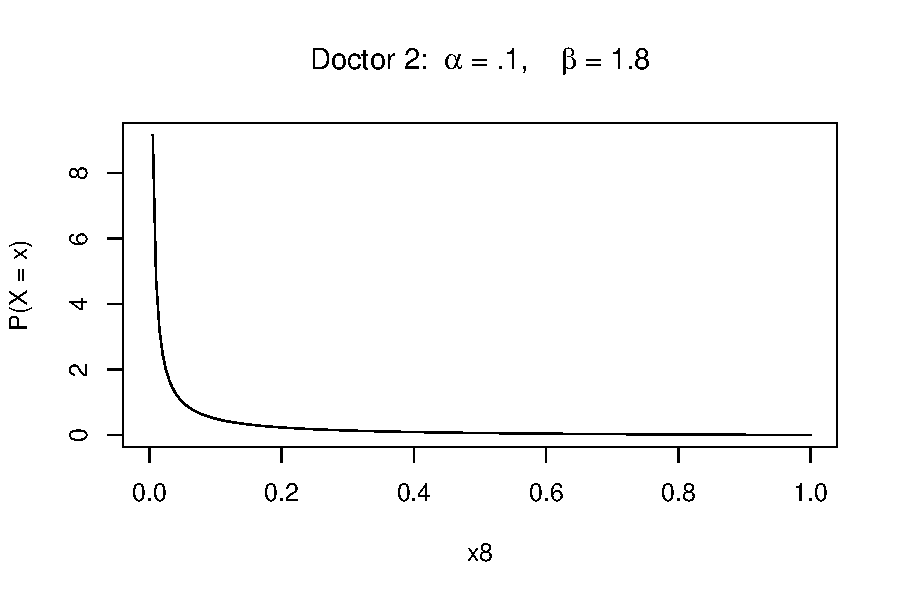
\includegraphics[width=\maxwidth]{figure/plot8b-1} 

}



\end{knitrout}

Now we plot the posteriors

\begin{knitrout}
\definecolor{shadecolor}{rgb}{0.969, 0.969, 0.969}\color{fgcolor}

{\centering 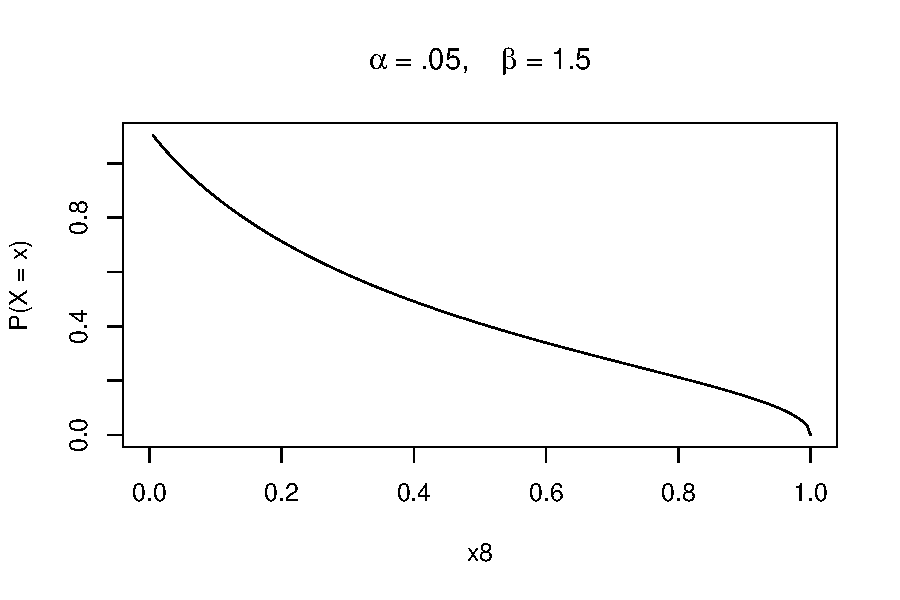
\includegraphics[width=\maxwidth]{figure/plot8c-1} 

}



\end{knitrout}

\begin{knitrout}
\definecolor{shadecolor}{rgb}{0.969, 0.969, 0.969}\color{fgcolor}

{\centering 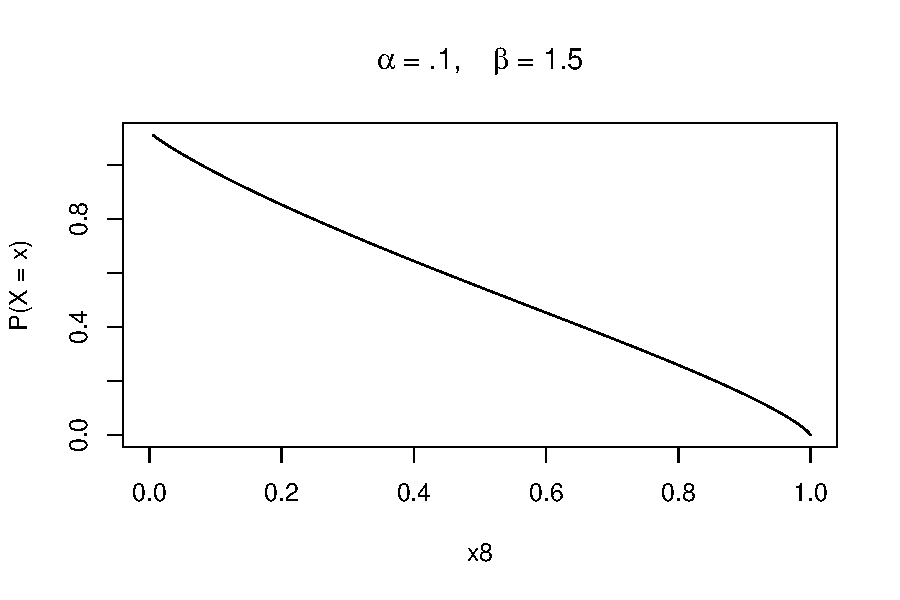
\includegraphics[width=\maxwidth]{figure/plot8d-1} 

}



\end{knitrout}
     
\end{enumerate}
\item Letting $X$ be the number of girls born and $\theta$ be the probability of any given birth being female, we have
\begin{align*}
P(\theta | X) & \propto P(X | \theta) P(\theta)\\
& = \underbrace{{493472 \choose 246945} ( \theta)^{246945} ( 1 - \theta)^{251526} \underset{(0,1)}{I(\theta)}}_{\text{Kernel of } Beta(246946, 251527)}
\end{align*}
So, with R, using the following code,
\begin{verbatim}
pbeta(.5, 246946, 251527)
\end{verbatim}
we can calculate $P(\theta < .5 | X) = 0.9999999999566463$. Thus, we can be 'morally certain' that $\theta < 0.5$.


\item 

For the poisson distribution, we have
\begin{align*}
L(\theta | x) &= \prod_{i=1}^n \frac{e^{- \theta} \theta^{x_i}}{x_i !}\\
&=  \frac{e^{- n \theta} \theta^{\sum_{i=1}^n x_i}}{\prod_{i=1}^n x_i !}\\
\end{align*}
giving

 \[ logL( \theta | x) =  - n \theta + \sum x_i log \theta - h(x) \]
 
so that 

\[ \dfrac{\partial log L (\theta | x)}{\partial \theta} = -n + \frac{\sum x_i}{\theta} \overset{set}{=} 0   \Longleftrightarrow \hat{\theta} = \bar{x} \]

Also, we have

\[ \dfrac{\partial^2 log L (\theta | x)}{\partial \theta^2} = - \frac{\sum x_i}{\theta^2} < 0 \]
giving us the max, and the fisher's information of 
\[ I (\theta) =  \frac{n}{\theta}  \]

Thus, a 95\% Wald type interval can be estimated as $\hat{\theta} \pm 1.96 ( \sqrt{\frac{\hat{\theta}}{n}})$

Similarly, for the binomial case, we have
\[ \hat{\theta} = \bar{x} \]

and 

\[ I(\theta) = \frac{n}{\theta ( 1 - \theta)} \]

giving the 95\% Wald interval as 

\[ \hat{\theta} \pm 1.96 \sqrt{\dfrac{\hat{\theta} (1 - \hat{\theta})}{n}} \]

For the Normal cases, we simply use the fact that $-2log(\lambda(x)) \overset{d}{\rightarrow} \chi^2_2$ and take the appropriate slice out of the contour for the 95th quantile.
\begin{enumerate}[label = (\alph*)]
\item We have 
\begin{knitrout}
\definecolor{shadecolor}{rgb}{0.969, 0.969, 0.969}\color{fgcolor}

{\centering 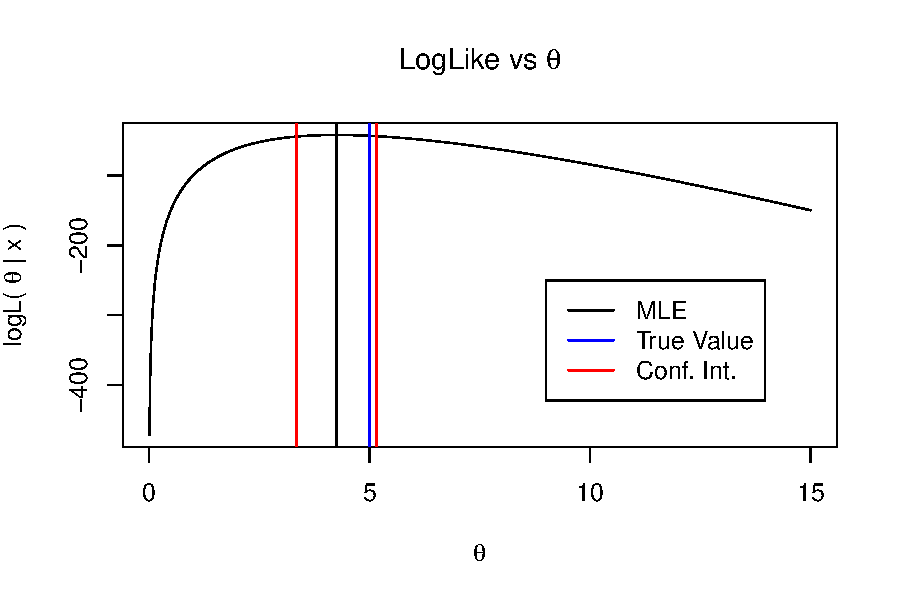
\includegraphics[width=\maxwidth]{figure/plot10a-1} 

}



\end{knitrout}
\item We have
\begin{knitrout}
\definecolor{shadecolor}{rgb}{0.969, 0.969, 0.969}\color{fgcolor}

{\centering 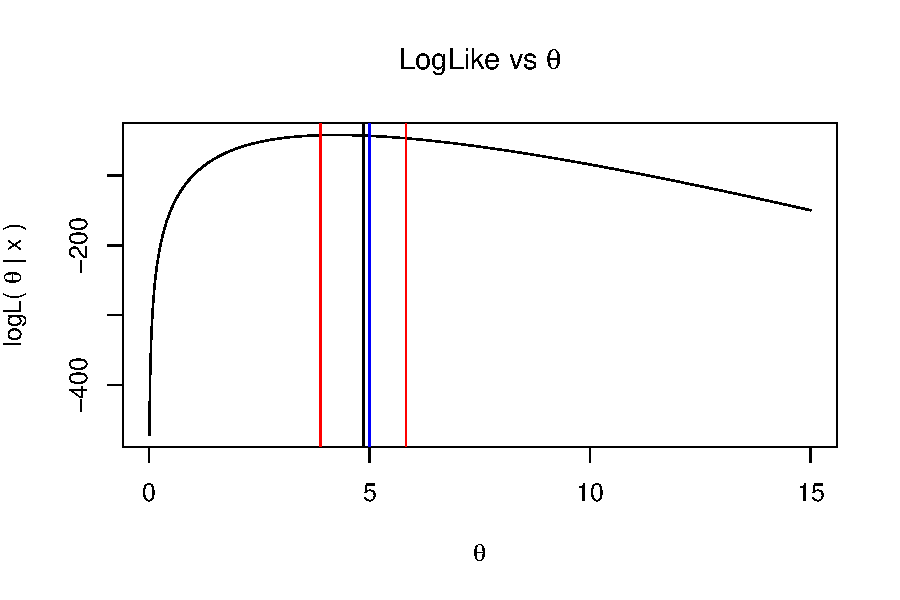
\includegraphics[width=\maxwidth]{figure/plot10b-1} 

}



\end{knitrout}
\item We have
\begin{knitrout}
\definecolor{shadecolor}{rgb}{0.969, 0.969, 0.969}\color{fgcolor}

{\centering 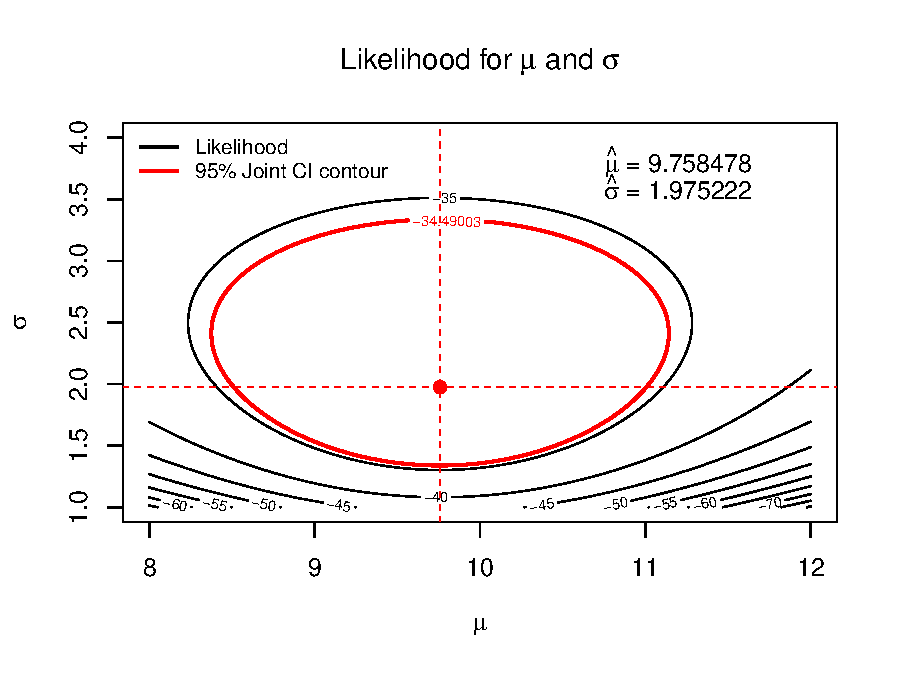
\includegraphics[width=\maxwidth]{figure/plot10c-1} 

}



\end{knitrout}
\item We have
\begin{knitrout}
\definecolor{shadecolor}{rgb}{0.969, 0.969, 0.969}\color{fgcolor}

{\centering 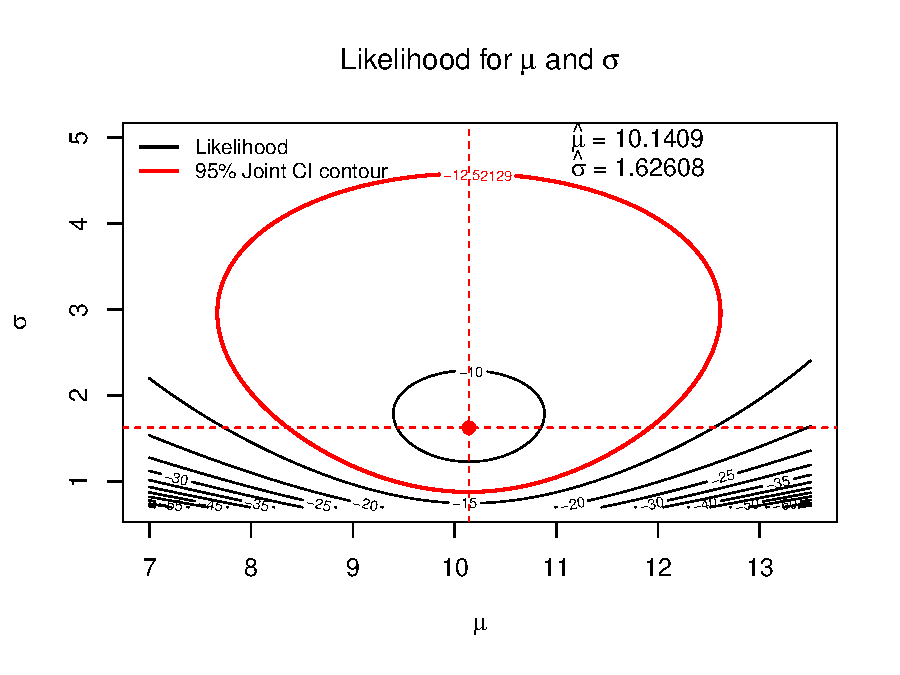
\includegraphics[width=\maxwidth]{figure/plot10d-1} 

}



\end{knitrout}

\item We have
\begin{knitrout}
\definecolor{shadecolor}{rgb}{0.969, 0.969, 0.969}\color{fgcolor}

{\centering 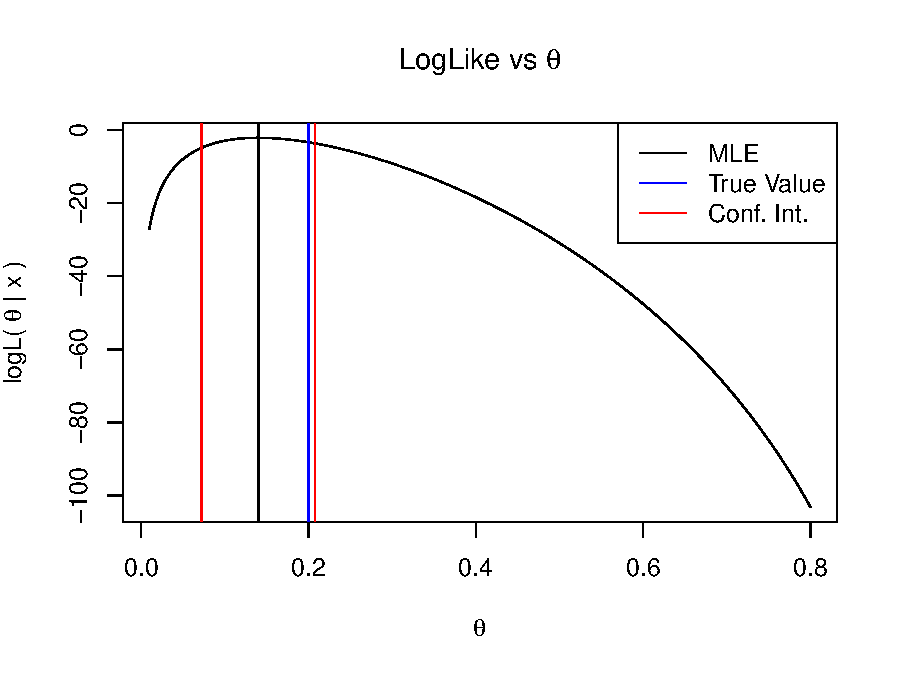
\includegraphics[width=\maxwidth]{figure/plot10e-1} 

}



\end{knitrout}

\item We have 
\begin{knitrout}
\definecolor{shadecolor}{rgb}{0.969, 0.969, 0.969}\color{fgcolor}

{\centering 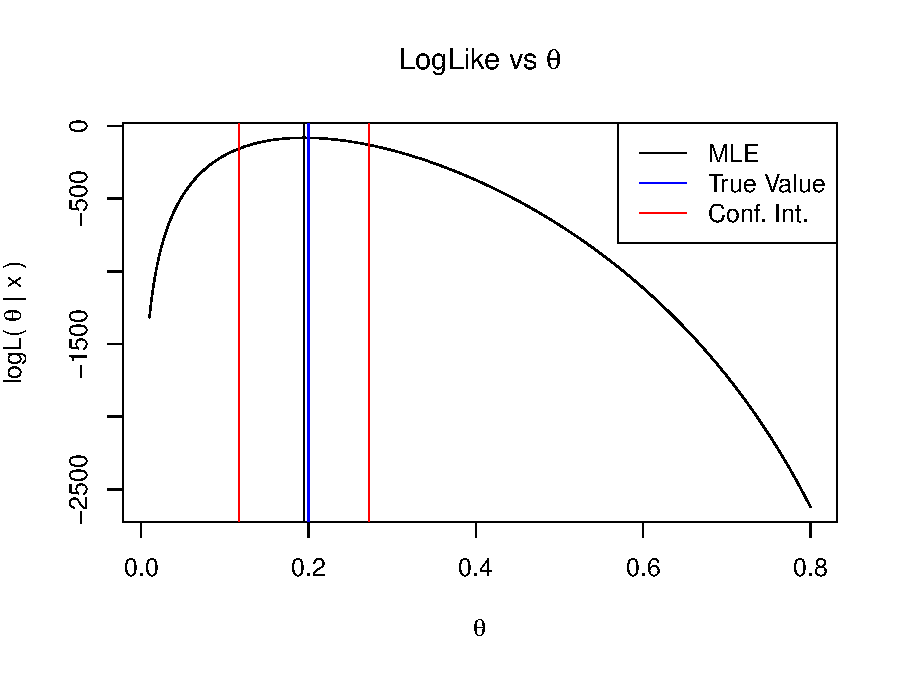
\includegraphics[width=\maxwidth]{figure/plot10f-1} 

}



\end{knitrout}
\item These plots of the MLE reinforce the fact that larger sample sizes are associated with smaller variances and less error. That is, that MLE's are asymptotically efficient. 
\end{enumerate}
\item 
\begin{enumerate}[label = (\alph*)]
\item We have
\begin{align*}
P(y) &= \sum_{i = 1}^2 p(y | \theta_i) p(\theta_i)\\
&= (\frac{1}{2})(\frac{1}{2 \sqrt{2 \pi}}) ( exp \{ - \frac{(y - 1)^2}{8} \} +  exp \{ - \frac{(y - 2)^2}{8} \})
\end{align*}
\item We have
\begin{align*}
P( \theta = 1 | y =1) &= \dfrac{p( \theta = 1) p( y = 1 | \theta = 1, \sigma = 2)}{p(y = 1)}\\
&= \dfrac{(\frac{1}{2})(\frac{1}{2 \sqrt{2 \pi}}) exp \{ 0 \}}{(\frac{1}{2}) ( \frac{1}{2 \sqrt{2 \pi}})(1 + exp \{ - \frac{1}{8} \})}\\
&= \dfrac{1}{1 + exp \{ -\frac{1}{8} \} }\\
& \approx 0.5312094
\end{align*}
\item To describe how the posterior changes as $\sigma$ changes, we plot the posterior as a function of $\sigma$. We have

\begin{knitrout}
\definecolor{shadecolor}{rgb}{0.969, 0.969, 0.969}\color{fgcolor}

{\centering 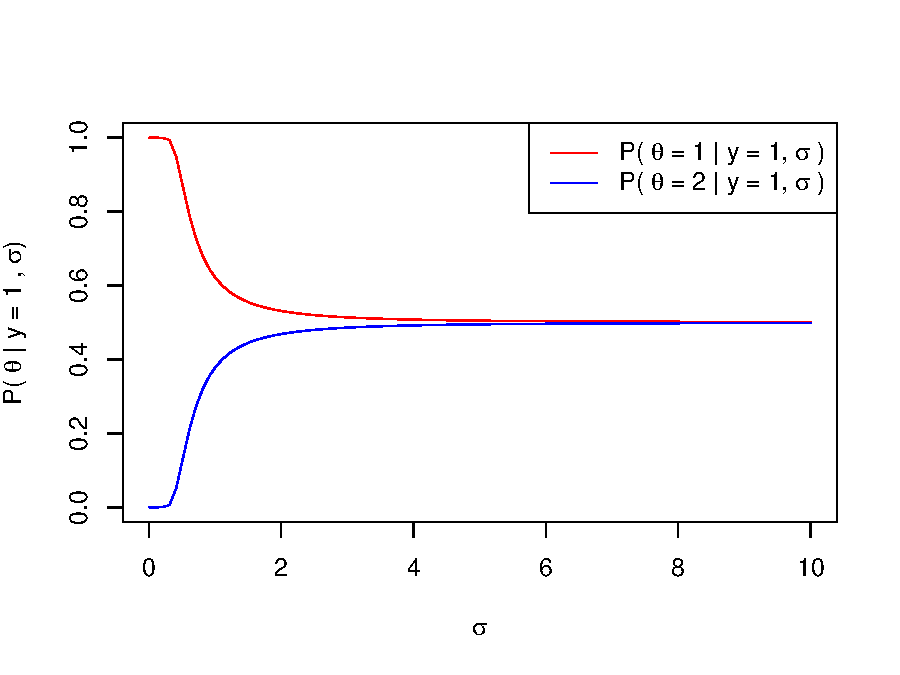
\includegraphics[width=\maxwidth]{figure/plot11c-1} 

}



\end{knitrout}
\end{enumerate}
\item We have
\begin{align*}
P(ident | twin \; bro) &= \dfrac{P(twin \; bro | ident) P(ident)}{P(twin \; bro | ident)P(ident) + P(twin \; bro| frat)P(frat)}\\
&= \dfrac{(\frac{1}{2})(\frac{1}{300})}{(\frac{1}{2})(\frac{1}{300}) + (\frac{1}{4})(\frac{1}{125})}\\
&= \frac{5}{11}\\
&=0.  \overline{45}
\end{align*}
\item 
\begin{enumerate}[label=(\alph*)]
\item
We have
\[ P_A(E) = P(E|I_A) = 1\]
or
\[ P_A(E) = P(E|I_A) = 0\]
depending on what outcome occured (1 if a 6 occured and 0 else). \\

We also have
\[ P_B(E) = P(E|I_B) = \frac{1}{6}\]

Hence, the probability of a rolling a '6' on a fair 6 sided die is subjective. However, this question does seem oddly worded. I think it should be stated "the probability of guessing the correct die after the die is rolled" for the above argument to be used. Certainly, a-prior, both person A and person B would agree that the probability of a '6' begin rolled is $\frac{1}{6}$, even if person A gets to see the outcome after the die is rolled.
\item
We have
\[ P_A(Brazil \; wins|I_A) \neq .5 \]
and we have
\[ P_B(Brazil \; wins|I_B) = .5 \]
Thus, the probability of Brazil winning the world cup is subjective.
\end{enumerate}
\item We have $y \sim Bin(n, \theta)$
\begin{enumerate}[label = (\alph*), start = 2]
\item We have
\begin{align*}
P(\theta | y) &\propto P(y | \theta) P(\theta)\\
& \propto { n \choose y} \theta^y(1 - \theta)^{n- y} \theta^{\alpha - 1} (1 - \theta)^{\beta - 1}\\
& \propto \underbrace{\theta^{y + \alpha - 1} (1 - \theta)^{n + \beta - y - 1}}_{\text{Kernel of } beta(y+ \alpha, n + \beta - y)}
\end{align*}
Thus, we have $E[ \theta | y] = \frac{ y + \alpha}{n + \beta - y + \alpha + y} = \frac{ y + \alpha}{n + \beta + \alpha}$\\

Suppose $\frac{y}{n} < \frac{\alpha}{\alpha + \beta}$
Then,
\begin{align*}
y &< \dfrac{n \alpha}{\alpha + \beta}\\
\Longleftrightarrow y + \alpha &< \dfrac{ \alpha ( n + \beta + \alpha)}{\alpha + \beta}\\
\Longleftrightarrow \dfrac{y + \alpha}{n + \beta + \alpha} &< \dfrac{\alpha}{\alpha + \beta}\\
\Longleftrightarrow \dfrac{y}{n} &< \dfrac{y + \alpha}{n + \beta + \alpha}
\end{align*}
and
\begin{align*}
y(\alpha + \beta) &< n \alpha \\
\Longleftrightarrow \beta y + \alpha y < n \alpha \\
\Longleftrightarrow y \alpha + y \beta + \alpha^2 + \alpha \beta & < n \alpha + \beta \alpha + \alpha^2 \\
\Longleftrightarrow \dfrac{y + \alpha}{n + \beta + \alpha} &< \dfrac{\alpha}{\alpha + \beta}
\end{align*}
Giving
\[ \dfrac{y}{n} < \dfrac{y + \alpha}{n + \beta + \alpha} <  \dfrac{\alpha}{\alpha + \beta} \]

Now, suppose $\frac{\alpha}{\alpha + \beta} < \frac{y}{n}$
We have
\begin{align*}
n \alpha & < y ( \alpha + \beta) \\
\Longleftrightarrow n \alpha & < \beta y + y \alpha\\
\Longleftrightarrow n y + n \alpha & < ny + \beta y + y \alpha\\
\Longleftrightarrow \dfrac{y + \alpha}{n + \beta + \alpha} &< \dfrac{y}{n}
\end{align*}
and we have
\begin{align*}
n \alpha &< y( \alpha + \beta)\\
\Longleftrightarrow n \alpha + \beta \alpha + \alpha^2 &< y \alpha + y \beta + \alpha^2 + \alpha \beta\\
\Longleftrightarrow \dfrac{ \alpha}{\alpha + \beta} &< \dfrac{y + \alpha}{n + \beta + \alpha}
\end{align*}
Giving
\[ \dfrac{\alpha}{\alpha + \beta} < \dfrac{y + \alpha}{n + \beta + \alpha} <  \dfrac{y}{n}\]
Thus showing $E[ \theta | y]$ is always between $\frac{\alpha}{\alpha + \beta}$ and $\frac{y}{n}$.
\item We have
\[ P( \theta | y) \propto P(y | \theta) P(\theta) = \underbrace{{n \choose y} \theta^y (1 -\theta)^{n - y} \underset{(0,1)}{I(\theta)}}_{\text{Kernel of } Beta(y + 1, n - y + 1)}   \]
and so 
\[ Var [ \theta | y] = \dfrac{(y + 1)(n - y + 1)}{(y + 1 + n - y + 1 ) (n + 2)^2} = \dfrac{- y^2 + ny + n +1}{(n + 2)^2(n + 3)} \]
Now, let's consider the extreme cases. If we let $y = n$ or $y = 0$, then we have
\[   Var [ \theta | y] =  \dfrac{n +1}{(n + 2)^2(n + 3)} < \dfrac{1}{12} \]
for all $n \geq 1$. For the in between cases, notice in the numerator that the first two terms would be negative. Thus, making the fraction even smaller than $\frac{1}{12}$ for all $n \geq 1$. Thus, we have that the posterior variance is always smaller than the prior variance.
\item
\end{enumerate}
\item
\begin{enumerate}[label = (\alph*)]
\item We have
\[ p( \phi) = 1 \underset{(0,1)}{I(\theta)} |h'(\theta) |^{-1} = \theta  \underset{(0,1)}{I(\theta)} \]
This is not obviously uninformative until you consider back transforming.

\item 
With 
\[ \theta | y \sim Pois( \theta) \]
we have 
\begin{align*}
P(y | \theta) &= \dfrac{e^{- \theta} \theta^y}{y !}\\
\Longrightarrow log P(\theta | y) &= - \theta + y log \theta + h(y)\\
\Longrightarrow \dfrac{ d log P(\theta |y)}{d \theta} & = - 1 + \dfrac{y}{\theta}\\
\Longrightarrow \dfrac{d^2 log P(\theta | y)}{d \theta^2} & = - \dfrac{y}{\theta^2}\\
\Longrightarrow J(\theta) &= - (- \dfrac{\theta}{\theta^2}) = \dfrac{1}{\theta}
\end{align*}
Thus, we have 
\[ P(\theta) \propto \theta^{- \frac{1}{2}} \]
\end{enumerate}
\item
\begin{enumerate}[label = (\alph*)]
\item In using the $Beta(0,0)$ prior, we have
\begin{align*}
P(\theta | x) & \propto P(x | \theta) p(\theta)\\
&= \underbrace{{6 \choose 2} \theta^2(1 - \theta)^4 (\theta)^{-1} (1-\theta)^{-1} \dfrac{1}{B(0,0)} \underset{(0,1)}{I(\theta)}}_{\text{Kernel of } Beta(2,4)}
\end{align*}
and so $\theta|x \sim Beta(2,4)$\\

Similarly, we can calculate as above that for the $Beta(.5,.5)$ prior, we have \\ $\theta | x \sim Beta(2.5, 4.5)$, for  the $Beta(1,1)$ prior, we have $\theta | x \sim Beta(3,5)$, and for the $Beta(2,2)$ prior, we have  $\theta| x \sim Beta(4,6)$. Below, plots of the posteriors for each case are given. 

\begin{knitrout}
\definecolor{shadecolor}{rgb}{0.969, 0.969, 0.969}\color{fgcolor}

{\centering 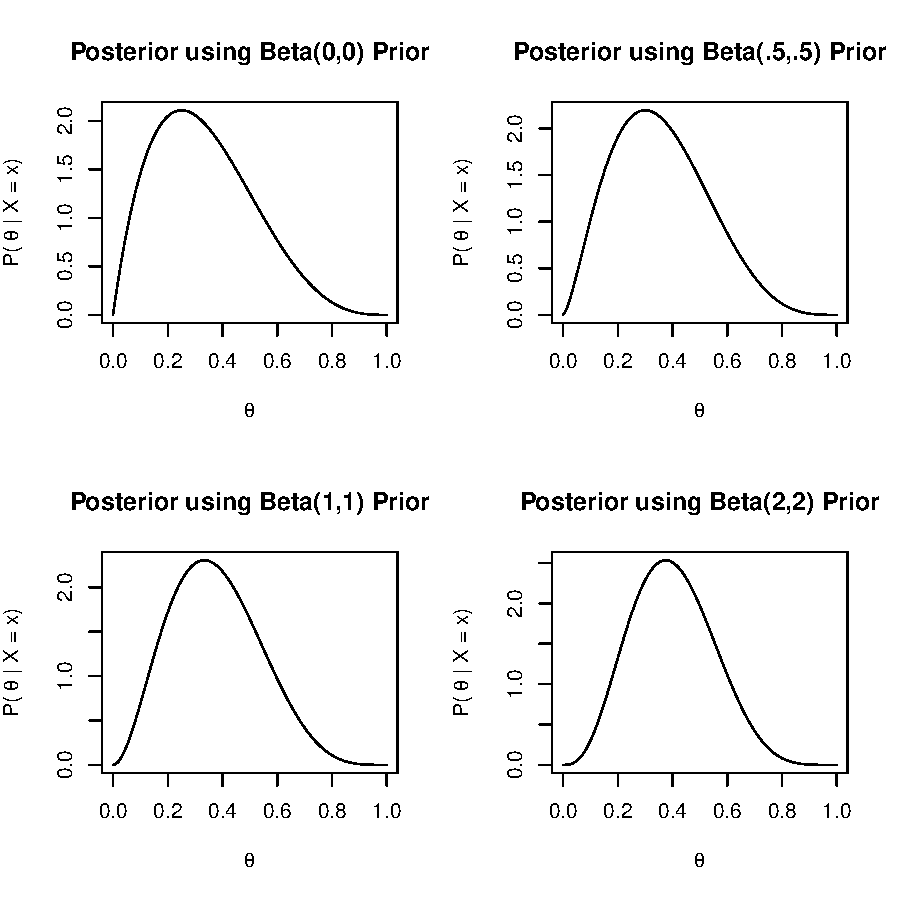
\includegraphics[width=\maxwidth]{figure/plot16a-1} 

}



\end{knitrout}
\item Using a similar calculation as in part (a), for the Beta(0,0) prior we have $\theta | x \sim  Beta(10,20)$, for the Beta(.5,.5) prior we have $\theta | x \sim Beta(10.5, 20.5)$, for the Beta(1,1) prior we have $\theta | x \sim Beta(11, 21)$, and for the $Beta(1,1)$ prior we have $\theta | x \sim Beta(12, 22)$. Plots for each posterior are given below. 
\begin{knitrout}
\definecolor{shadecolor}{rgb}{0.969, 0.969, 0.969}\color{fgcolor}

{\centering 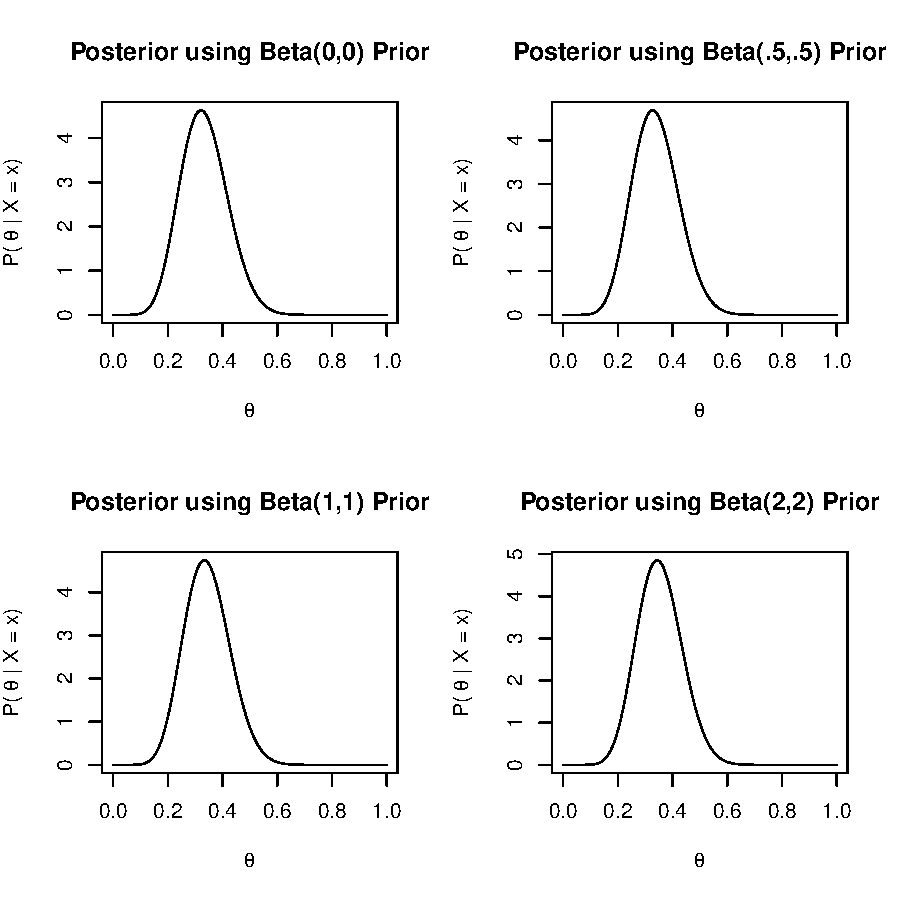
\includegraphics[width=\maxwidth]{figure/plot16b-1} 

}



\end{knitrout}
\item
For the Beta(0,0) prior we have $\theta | x \sim  Beta(30,60)$, for the Beta(.5,.5) prior we have $\theta | x \sim Beta(30.5, 60.5)$, for the Beta(1,1) prior we have $\theta | x \sim Beta(31, 61)$, and for the $Beta(1,1)$ prior we have $\theta | x \sim Beta(32, 62)$. Plots for each posterior are given below. 
\begin{knitrout}
\definecolor{shadecolor}{rgb}{0.969, 0.969, 0.969}\color{fgcolor}

{\centering 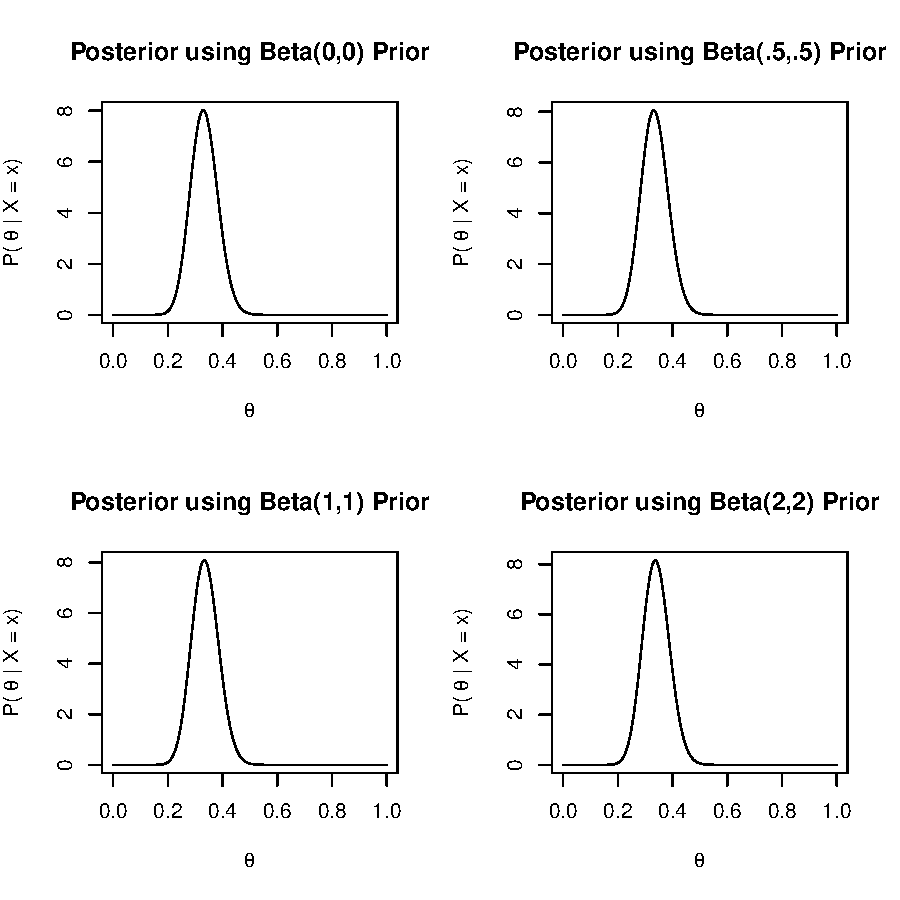
\includegraphics[width=\maxwidth]{figure/plot16c-1} 

}



\end{knitrout}

From parts (a) thru (c), we see that even though our sample proportion stays the same, we see that the effect of the prior on the posterior decreases as sample size increases (evident in how similar the posterior distributions are for the various given priors for larger sample sizes as opposed to the smaller sample size in part (a)). Additionally, we see that as sample size increases, the data has a greater influence on the posterior (evident in the decrease in spread in the posterior going from (a) to (c)). We also see that $\hat{\theta} \overset{p}{\rightarrow} \theta$
\end{enumerate}
\item "Subjective" simply means that two people could reasonably arrive at differing conclusions in a process in contrast to "objective" where they ought to arrive at the same conclusion.\\

\begin{itemize}
\item
Research question formulation : Subjective \\

 Many researcher's may ask the same question in a different manner. For instance, different disciplines may have some overlap, but describe the question in a different framework.\\

\item Experimental Design \\

Researchers also might use different experimental designs for based on their beliefs in prior parameter  estimates. They also might, in an observational study, choose one dataset over another. They might choose one over the other based on how well each represents a natural experiment. \\


\item Model Formulation : Subjective \\

Initial models considered as well as model selection methodologies may reasonably vary among researchers both based on subject matter expertise, as well as various cutoff's one might make. One researcher might view a p-value of .09 as meaningful while another might not. Also, researchers might reasonably differ in modeling approaches. One might want to go with Bayesian inference while another might want to use a frequentist approach. This could also influence the model selection that one might be willing to make as well. Both could be argued for being reasonable. \\

\item Model Calculation : Subjective\\

Different researchers might use different algorithms (software) on the same problem based on their concerns about how the various algorithms will perform on the dataset. 

\item Dissemination of Statements : Subjective\\

Researchers might disagree on how to interpret the statistical results in the context of the problem. For instance, the scope of inference one researcher might be willing to make may be different than another based on ignorability assumptions each is willing to make. 

\end{itemize}
\item $\checkmark$
\end{enumerate}
\newpage
\section*{R-Code}
\begin{verbatim}


## 6

x6 <- seq(0,1, length = 200)

# alpha = beta = .5
plot(x6, dbeta(x6,.5,.5), type = "l", 
     main = expression(paste(alpha," = ", beta," = .5")),
     ylab = "P(X = x)") 

# alpha = beta = 1
plot(x6, dbeta(x6,1,1), type = "l", 
     main = expression(paste(alpha," = ", beta," = 1")),
     ylab = "P(X = x)")  

# alpha = beta = 2
plot(x6, dbeta(x6,2,2), type = "l", 
     main = expression(paste(alpha," = ", beta," = 2")),
     ylab = "P(X = x)")  

# alpha = beta = 10
plot(x6, dbeta(x6,10,10), type = "l", 
     main = expression(paste(alpha," = ", beta," = 10")),
     ylab = "P(X = x)")  

##7
x7 <- seq(0,4, length = 200)

# alpha = beta = .5
plot(x7, dgamma(x7,.5,.5), type = "l", 
     main = expression(paste(alpha," = ", beta," = .5")),
     ylab = "P(X = x)") 

# alpha = beta = 1
plot(x7, dgamma(x7,1,1), type = "l", 
     main = expression(paste(alpha," = ", beta," = 1")),
     ylab = "P(X = x)")  

# alpha = beta = 2
plot(x7, dgamma(x7,2,2), type = "l", 
     main = expression(paste(alpha," = ", beta," = 2")),
     ylab = "P(X = x)")  

# alpha = beta = 10
plot(x7, dgamma(x7,10,10), type = "l", 
     main = expression(paste(alpha," = ", beta," = 10")),
     ylab = "P(X = x)")  

## 8
#a
# Doctor 1
(.92)*(.05)/((.92)*(.05) + (.1)*(.95))

# Doctor 2
(.92)*(.1)/((.92)*(.1) + (.1)*(.90))

#b

# Prior quantiles

quants <- c(.01, .05, seq(.1, 1, by = .1))
quants

# Doctor 1
d1_quant <- pbeta(quants, .05, 1.5)
d1_quant

#Doctor 2
d2_quant <- pbeta(quants, .1, 1.8)
d2_quant

##Prior Plots

#Doctor 1
x8 <- seq(0,1, length = 200)
plot(x8, dbeta(x8,.05, 1.5), type = "l", 
     main = expression(paste("Doctor 1:  ", alpha," = .05,    ", beta," = 1.5")),
     ylab = "P(X = x)") 

#Doctor 2
plot(x8, dbeta(x8,.06, 2), type = "l", 
     main = expression(paste("Doctor 2:  ", alpha," = .1,    ", beta," = 1.8")),
     ylab = "P(X = x)") 

## Posterior Plots

# Doctor 1
doc_1_post <- ((.92)*dbeta(x8, .05, 1.5))/((.92)*dbeta(x8, .05, 1.5) + 
              (.1)*(1 - dbeta(x8, .05, 1.5)))
plot(x8, doc_1_post, type = "l", 
     main = expression(paste(alpha," = .05,    ", beta," = 1.5")),
     ylab = "P(X = x)")

#mean(sample(x8, size = 10000, replace = TRUE, prob = doc_1_post))


# Doctor 2
doc_2_post <- ((.92)*dbeta(x8, .1, 1.8))/((.92)*dbeta(x8, .1, 1.8) + 
              (.1)*(1 - dbeta(x8, .1, 1.8)))
plot(x8, doc_2_post, type = "l", 
     main = expression(paste(alpha," = .1,    ", beta," = 1.5")),
     ylab = "P(X = x)")

#mean(sample(x8, size = 10000, replace = TRUE, prob = doc_2_post))

x8b <- seq(0.001,1, length = 200)


# alpha = beta = .5
plot(x8b, dbeta(x8b,.1,5), type = "l", 
     main = expression(paste(alpha," = .1,    ", beta," = 2")),
     ylab = "P(X = x)") 
prior_a <- dbeta(x8b, .1, 1.65)
doc_a_post <- ((.92)*prior_a)/((.92)*prior_a + (.08)*(1 - prior_a))
doc_a_post[1] = 0
plot(x8b, doc_a_post, type = "l", 
     main = expression(paste(alpha," = .03,    ", beta," = 2")),
     ylab = "P(X = x)")

#mean(sample(x8b, size = 10000, replace = TRUE, prob = doc_a_post))

## 9 
options(digits = 16)
pbeta(.5, 246946, 251527)

##10

#a
set.seed(2015)
data_10a <- rpois(20, 5)
data_10a
mean(data_10a)
POIS_LL <- function(theta) sum(dpois(data_10a, theta, log = TRUE))
POIS_LL_neg <- function(theta) - sum(dpois(data_10a, theta, log = TRUE))
nlm(POIS_LL_neg, 4 , gradtol = 1e-16)$est
ndim = 1000
grid.theta <- matrix(seq(0.01,15, length.out = ndim), 1, ndim)
logL_vals <- apply(grid.theta, 2, POIS_LL)

plot(grid.theta, logL_vals, type = "l", 
     ylab = expression(paste("logL( ", theta, " | x )")),
     xlab = expression(theta), main = expression(paste("LogLike vs ", theta)))
abline(v = nlm(POIS_LL_neg, 4 , gradtol = 1e-16)$est, col = "black")
abline(v = 5, col = "blue")
abline(v = mean(data_10a) - qnorm(.975) * sqrt(mean(data_10a) / 20), col = "red")
abline(v = mean(data_10a) + qnorm(.975) * sqrt(mean(data_10a) / 20), col = "red")
legend(9, -250, c("MLE", "True Value", "Conf. Int."), 
       col = c("black", "blue", "red"), lty = 1)

#b
set.seed(2015)
data_10b <- rpois(100, 5)
data_10b
mean(data_10b)
POIS_LL_10b <- function(theta) sum(dpois(data_10b, theta, log = TRUE))
POIS_LL_neg_10b <- function(theta) - sum(dpois(data_10b, theta, log = TRUE))
nlm(POIS_LL_neg_10b, 4 , gradtol = 1e-16)$est
ndim = 10000
grid.theta <- matrix(seq(0.01,15, length.out = ndim), 1, ndim)
logL_vals <- apply(grid.theta, 2, POIS_LL)

plot(grid.theta, logL_vals, type = "l", 
     ylab = expression(paste("logL( ", theta, " | x )")),
     xlab = expression(theta), main = expression(paste("LogLike vs ", theta)))
abline(v = nlm(POIS_LL_neg_10b, 4 , gradtol = 1e-16)$est, col = "black")
abline(v = 5, col = "blue")
abline(v = mean(data_10b) - qnorm(.975) * sqrt(mean(data_10b) / 20), col = "red")
abline(v = mean(data_10b) + qnorm(.975) * sqrt(mean(data_10b) / 20), col = "red")
legend(9, -850, c("MLE", "True Value", "Conf. Int."), 
       col = c("black", "blue", "red"), lty = 1)

#c
set.seed(2015)
data_10c <- rnorm(15, 10, sqrt(5))

NORM_LL <- function(mu, sigma) sum(dnorm(data_10c, mu, sigma, log = TRUE))
NORM_LL_p <- function(p) - NORM_LL(p[1], p[2])

#obtain MLE's
out.NORM <- nlm(NORM_LL_p, c(8, 3))
out.NORM
# Check w/ Theoreticals
mean(data_10c)
sqrt(sum((data_10c - mean(data_10c))^2)/15)

#generate grid of values
ndim = 300
mu <- seq(8,12, length.out = ndim)
sigma <- seq(1,4,length.out = ndim)
grid_val_10c <- expand.grid(mu, sigma)

# Likelihoods over grid
z <- -apply(grid_val_10c,1,NORM_LL_p)

#make z back into a matrix
zmat <- matrix(z, nrow=ndim)

## confidence interval likelihood level
lower.limit <- -out.NORM$minimum-.5*qchisq(.95,2)

# Draw Likelihood Surface
contour(mu, sigma, zmat, xlab=expression(mu), ylab=expression(sigma),
        main = expression(paste("Likelihood for ", mu, " and ", sigma)))
#add MLE to graph
points(out.NORM$estimate[1], out.NORM$estimate[2], pch=16, col=2, cex=1.2)
contour(mu, sigma, zmat, xlab=expression(mu), 
        ylab=expression(theta), levels= lower.limit, lty=1, col="red", 
        lwd=2, add = TRUE)
legend('topleft', c("Likelihood", "95% Joint CI contour"), lty=1, col=c(1,"red"),
        lwd=c(2,2), bty='n', cex=.8)
abline(v=out.NORM$estimate[1], col=2, lty=2)
abline(h=out.NORM$estimate[2], col=2, lty=2)
text(11.2,3.8, expression(paste(hat(mu), " = 9.758478")))
text(11.2,3.6, expression(paste(hat(sigma), " = 1.975222")))

#d
set.seed(2009)
data_10d <- rnorm(5, 10, sqrt(5))

NORM_LL <- function(mu, sigma) sum(dnorm(data_10d, mu, sigma, log = TRUE))
NORM_LL_p <- function(p) - NORM_LL(p[1], p[2])

#obtain MLE's
out_NORM_10d <- nlm(NORM_LL_p, c(8, 3))
out_NORM_10d
# Check w/ Theoreticals
mean(data_10d)
sqrt(sum((data_10d - mean(data_10d))^2)/5)

#generate grid of values
ndim = 300
mu <- seq(7,13.5, length.out = ndim)
sigma <- seq(.7,5,length.out = ndim)
grid_val_10d <- expand.grid(mu, sigma)

# Likelihoods over grid
z <- -apply(grid_val_10d,1,NORM_LL_p)

#make z back into a matrix
zmat <- matrix(z, nrow=ndim)

## confidence interval likelihood level
lower.limit <- -out_NORM_10d$minimum-.5*qchisq(.95,2)

# Draw Likelihood Surface
contour(mu, sigma, zmat, xlab=expression(mu), ylab=expression(sigma),
        main = expression(paste("Likelihood for ", mu, " and ", sigma)))
#add MLE to graph
points(out_NORM_10d$estimate[1], out_NORM_10d$estimate[2], pch=16, col=2, cex=1.2)
contour(mu, sigma, zmat, xlab=expression(mu), 
        ylab=expression(theta), levels= lower.limit, lty=1, col="red", lwd=2, add = TRUE)
legend('topleft', c("Likelihood", "95% Joint CI contour"), lty=1, col=c(1,"red"), 
       lwd=c(2,2), bty='n', cex=.8)
abline(v=out_NORM_10d$estimate[1], col=2, lty=2)
abline(h=out_NORM_10d$estimate[2], col=2, lty=2)
text(11.8,5, expression(paste(hat(mu), " = 10.1409")))
text(11.8, 4.7, expression(paste(hat(sigma), " = 1.62608")))

# e
set.seed(2015)
data_10e <- rbinom(1, 100, .2)
data_10e
data_10e/100
BINOM_LL <- function(theta) sum(dbinom(data_10e, 100, theta, log = TRUE))
BINOM_LL_neg <- function(theta) - sum(dbinom(data_10e, 100, theta, log = TRUE))
out_BIN_10e <- nlm(BINOM_LL_neg, .2, stepmax = .08)

ndim = 10000
grid.theta <- matrix(seq(0.01,.8, length.out = ndim), 1, ndim)
logL_vals_10e <- apply(grid.theta, 2, BINOM_LL)

plot(grid.theta, logL_vals_10e, type = "l", 
     ylab = expression(paste("logL( ", theta, " | x )")),
     xlab = expression(theta), main = expression(paste("LogLike vs ", theta)))
abline(v = out_BIN_10e$est, col = "black")
abline(v = .2, col = "blue")
abline(v = data_10e/100 - qnorm(.975) * 
       sqrt((data_10e/100)*(1 - data_10e/100) / 100), col = "red")
abline(v = data_10e/100 + qnorm(.975) * 
       sqrt((data_10e/100)*(1 - data_10e/100) / 100), col = "red")
legend('topright', c("MLE", "True Value", "Conf. Int."), 
       col = c("black", "blue", "red"), lty = 1)

# f
set.seed(2015)
data_10f <- rbinom(30, 100, .2)
data_10f
mean(data_10f)/100
BINOM_LL_10f <- function(theta) sum(dbinom(data_10f, 100, theta, log = TRUE))
BINOM_LL_neg_10f <- function(theta) - sum(dbinom(data_10f, 100, theta, log = TRUE))
out_BIN_10f <- nlm(BINOM_LL_neg_10f, .2, stepmax = .08)

ndim = 10000
grid.theta <- matrix(seq(0.01,.8, length.out = ndim), 1, ndim)
logL_vals_10f <- apply(grid.theta, 2, BINOM_LL_10f)

plot(grid.theta, logL_vals_10f, type = "l", 
    ylab = expression(paste("logL( ", theta, " | x )")),
     xlab = expression(theta), main = expression(paste("LogLike vs ", theta)))
abline(v = out_BIN_10f$est, col = "black")
abline(v = .2, col = "blue")
abline(v = mean(data_10f)/100 - qnorm(.975) * 
       sqrt((mean(data_10f)/100)*(1 - mean(data_10f)/100) / 100), col = "red")
abline(v = mean(data_10f)/100 + qnorm(.975) * 
       sqrt((mean(data_10f)/100)*(1 - mean(data_10f)/100) / 100), col = "red")
legend('topright', c("MLE", "True Value", "Conf. Int."),
       col = c("black", "blue", "red"), lty = 1)


## 11

# b
1/(1+exp(-8))

# c
f_x_1 <- function(x) 1/(1+exp(-(1/(2*(x^2)))))

p_theta_1 <- f_x_1(seq(.01, 10, length.out = 100))
p_theta_2 <- 1 - p_theta_1

plot(seq(.01, 10, length.out = 100), p_theta_1, type = "l", ylim = c(0,1), 
     col = "red", xlab = expression(sigma),
    ylab = expression(paste("P( ", theta, " | y = 1 , ", sigma, ")")))
lines(seq(.01, 10, length.out = 100), p_theta_2, type = "l", col = "blue")
legend('topright', 
       c(expression(paste("P( ",theta, " = 1 | y = 1, ", sigma, " )")), 
        expression(paste("P( ",theta, " = 2 | y = 1, ", sigma, " )"))),
       col = c( "red", "blue"), lty = 1)

## 16 
# a 
x_16 <- seq(0,1, length.out = 200)
par(mfrow = c(2,2))
plot(x_16, dbeta(x_16, 2,4), type = "l",
     xlab = expression(theta), ylab = expression(paste("P( ", theta, " | X = x)")),
     main = "Posterior using Beta(0,0) Prior")
plot(x_16, dbeta(x_16, 2.5,4.5), type = "l",
     xlab = expression(theta), ylab = expression(paste("P( ", theta, " | X = x)")),
     main = "Posterior using Beta(.5,.5) Prior")
plot(x_16, dbeta(x_16, 3,5), type = "l",
     xlab = expression(theta), ylab = expression(paste("P( ", theta, " | X = x)")),
     main = "Posterior using Beta(1,1) Prior")
plot(x_16, dbeta(x_16, 4,6), type = "l",
     xlab = expression(theta), ylab = expression(paste("P( ", theta, " | X = x)")),
     main = "Posterior using Beta(2,2) Prior")

# b
x_16 <- seq(0,1, length.out = 200)
par(mfrow = c(2,2))
plot(x_16, dbeta(x_16, 10,20), type = "l",
     xlab = expression(theta), ylab = expression(paste("P( ", theta, " | X = x)")),
     main = "Posterior using Beta(0,0) Prior")
plot(x_16, dbeta(x_16, 10.5,20.5), type = "l",
     xlab = expression(theta), ylab = expression(paste("P( ", theta, " | X = x)")),
     main = "Posterior using Beta(.5,.5) Prior")
plot(x_16, dbeta(x_16, 11,21), type = "l",
     xlab = expression(theta), ylab = expression(paste("P( ", theta, " | X = x)")),
     main = "Posterior using Beta(1,1) Prior")
plot(x_16, dbeta(x_16, 12,22), type = "l",
     xlab = expression(theta), ylab = expression(paste("P( ", theta, " | X = x)")),
     main = "Posterior using Beta(2,2) Prior")

# c
x_16 <- seq(0,1, length.out = 200)
par(mfrow = c(2,2))
plot(x_16, dbeta(x_16, 30,60), type = "l",
     xlab = expression(theta), ylab = expression(paste("P( ", theta, " | X = x)")),
     main = "Posterior using Beta(0,0) Prior")
plot(x_16, dbeta(x_16, 30.5,60.5), type = "l",
     xlab = expression(theta), ylab = expression(paste("P( ", theta, " | X = x)")),
     main = "Posterior using Beta(.5,.5) Prior")
plot(x_16, dbeta(x_16, 31,61), type = "l",
     xlab = expression(theta), ylab = expression(paste("P( ", theta, " | X = x)")),
     main = "Posterior using Beta(1,1) Prior")
plot(x_16, dbeta(x_16, 32,62), type = "l",
     xlab = expression(theta), ylab = expression(paste("P( ", theta, " | X = x)")),
     main = "Posterior using Beta(2,2) Prior")

\end{verbatim}
\end{document})
